\documentclass[class=report, crop=false, 12pt,a4paper]{standalone}
\usepackage{enumitem}
\usepackage{multicol}
\usepackage{graphicx}
\usepackage{float}
\usepackage{amsmath}
\usepackage{amssymb}
\usepackage{mathtools}
\usepackage{siunitx}
\usepackage{commath}
\usepackage{array}
\usepackage{natbib}
\usepackage{tikz}
\usepackage[a4paper,width=150mm,top=25mm,bottom=25mm]{geometry}
\usetikzlibrary{positioning, fit, calc}   
\tikzset{block/.style={draw, thick, text width=3cm ,minimum height=1.3cm, align=center},   
line/.style={-latex}     
}  
\setlength{\parindent}{0pt}
\begin{document}
\section{Conformal mapping}
\subsection{Joukowsky Transformation}
The question is how can we transform our cylinder into something that looks like an airfoil? We achieve this by using conformal mapping which maps each part of our coordinate space to a new one. 
\begin{align}
  x &= r\cos{\theta}\\
  y &= r\sin{\theta}\\
  w &= G(z) = z + \frac{\lambda^2}{z}\\
  z &= re^{i\theta} = x + yi\\
  w &= \zeta + \xi i
\end{align}
\begin{figure}[H]
  \centering
  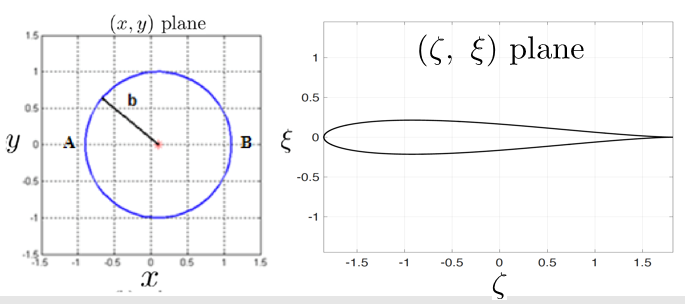
\includegraphics[width = 0.9\textwidth]{../img/diagram32.png}
\end{figure}
\subsection{Flat plate and Ellipse}
Lets consider a cylinder:
\begin{figure}[H]
  \centering
  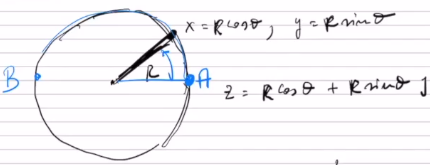
\includegraphics[width = 0.9\textwidth]{../img/diagram33.png}
\end{figure}
\begin{align}
  z &= R\cos{\theta} + Ri\sin{\theta}\\
  w &= G(z) = z + \frac{\lambda^2}{z}\\
  &=  R\cos{\theta} + Ri\sin{\theta} + \frac{\lambda^2}{R\cos{\theta} + Ri\sin{\theta}}\\
  &= R\cos{\theta} + Ri\sin{\theta} + \frac{\lambda^2 (R\cos{\theta} - Ri\sin{\theta})}{(R\cos{\theta} + Ri\sin{\theta})(R\cos{\theta} - Ri\sin{\theta})}\\
  &= R\cos{\theta} + Ri\sin{\theta} + \frac{\lambda^2 (R\cos{\theta} - Ri\sin{\theta})}{R^2}\\
  w &= R\cos{\theta} \left(1 + \frac{\lambda^2}{R}\right) + Ri\sin{\theta} \left(1 - \frac{\lambda^2}{R}\right)
\end{align}
When $\lambda = R$, we achieve a flat plate transformation as our imaginary term is always 0. When $\lambda \neq R$, we achieve an elliptical shape.
\begin{figure}[H]
  \centering
  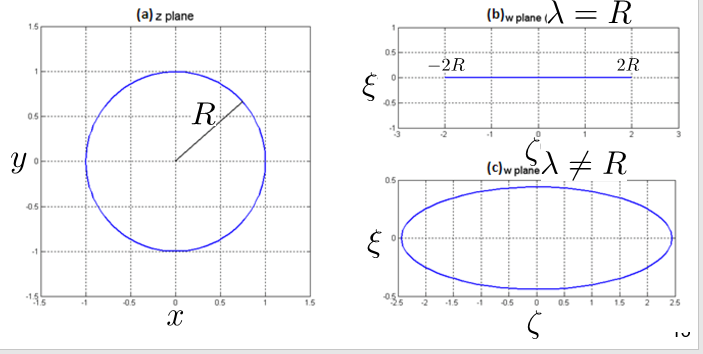
\includegraphics[width = 0.9\textwidth]{../img/diagram34.png}
\end{figure}
\subsection{Aerofoils}
We can further refine our conformal mapping by adding two elements to our equation, $x_c$ and $y_c$. These two terms effect the center of the cylinder in $x$ and $y$. 
\begin{gather}
  w = G(z) = z + \frac{\lambda^2}{z}\\
  \lambda = R - \sqrt{x_c^2 + y_c^2}\\
  z = x + x_c + (y + y_c)i \rightarrow w = \zeta + \xi i
\end{gather}
Mapping these into their respective planes:
\begin{align}
  x_c &\neq 0\\
  y_c &= 0
\end{align}
\begin{figure}[H]
  \centering
  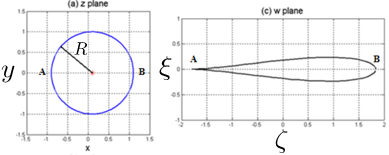
\includegraphics[width = 0.7\textwidth]{../img/diagram35.png}
\end{figure}
\begin{align}
  x_c &\neq 0\\
  y_c &\neq 0 
\end{align}
\begin{figure}[H]
  \centering
  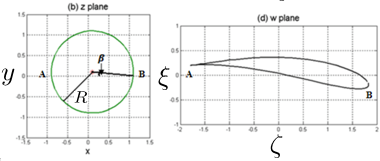
\includegraphics[width = 0.7\textwidth]{../img/diagram36.png}
\end{figure}
\section{Uniform stream + circulation}
What is the correct relationship between the circulation and the angle of incidence?
\begin{align}
  \Gamma &= f(\alpha)\\
  \textrm{Stagnation points: } u_r &= 0, \ u_\theta = 0\\
  \phi &= V_\infty r \cos{(\theta - \alpha)}\left(1 + \frac{R^2}{r^2}\right) - \frac{\Gamma}{2\pi}\theta\\
  \psi &= V_\infty r \sin{(\theta - \alpha)}\left(1 - \frac{R^2}{r^2}\right) + \frac{\Gamma}{2\pi} \log{\left(\frac{r}{R}\right)}
\end{align}
\begin{figure}[H]
  \centering
  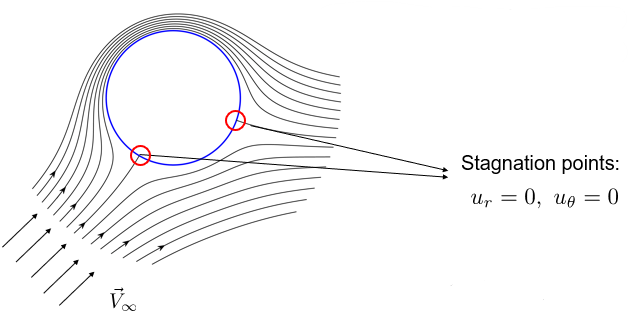
\includegraphics[width = 0.7\textwidth]{../img/diagram37.png}
\end{figure}
\section{Kutta condition}
I can apply the Joukowsky Transformation to the streamlines around the cylinder and obtain the streamlines around the airfoil. However I need to carefully select the circulation, $\Gamma$.
\begin{figure}[H]
  \centering
  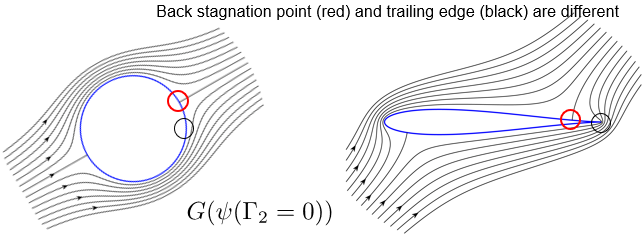
\includegraphics[width = 0.9\textwidth]{../img/diagram38.png}
\end{figure}
We can see that this streamline is unrealistic. This is because to curl around the trailing edge cusp, the speed goes to infinity. This is clearly impossible and flow separation would occur instead. This is the wrong circulation value for the given angle of incidence.
\begin{figure}[H]
  \centering
  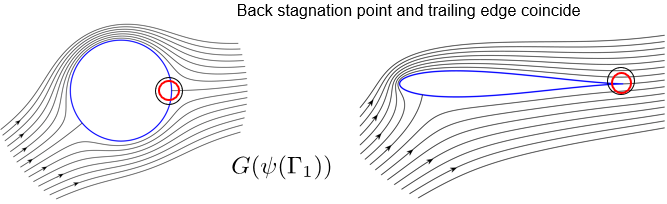
\includegraphics[width = 0.9\textwidth]{../img/diagram39.png}
\end{figure}
This streamline is more realistic as the velocity is parallel to the trailing edge cusp and its component in the vertical direction is zero. This circulation can be used to predict the lift $F_L$ but still predicts no drag $(F_D = 0)$.
\end{document}